\documentclass[12pt, a4paper, titlepage]{article}
\usepackage[spanish]{babel}
\usepackage[utf8]{inputenc}
\usepackage{pdflscape}
\usepackage{geometry}
\usepackage{pdfpages}
\usepackage{listings}
\usepackage{color}
\usepackage{textcomp}
\usepackage{verbatim}
\usepackage[colorlinks=true,linkcolor=black]{hyperref}
% Definimos JS en listings para que pueda colorearlo :)

\lstdefinelanguage{JavaScript}{
  morekeywords=[1]{break, continue, delete, else, for, function, if, in,
    new, return, this, typeof, var, void, while, with},
  % Literals, primitive types, and reference types.
  morekeywords=[2]{false, null, true, boolean, number, undefined,
    Array, Boolean, Date, Math, Number, String, Object},
  % Built-ins.
  morekeywords=[3]{eval, parseInt, parseFloat, escape, unescape},
  sensitive,
  morecomment=[s]{/*}{*/},
  morecomment=[l]//,
  morecomment=[s]{/**}{*/}, % JavaDoc style comments
  morestring=[b]',
  morestring=[b]"
}[keywords, comments, strings]

\definecolor{mediumgray}{rgb}{0.3, 0.4, 0.4}
\definecolor{mediumblue}{rgb}{0.0, 0.0, 0.8}
\definecolor{forestgreen}{rgb}{0.13, 0.55, 0.13}
\definecolor{darkviolet}{rgb}{0.58, 0.0, 0.83}
\definecolor{royalblue}{rgb}{0.25, 0.41, 0.88}
\definecolor{crimson}{rgb}{0.86, 0.8, 0.24}

\lstdefinestyle{JSES6Base}{
  backgroundcolor=\color{white},
  basicstyle=\ttfamily,
  breakatwhitespace=false,
  breaklines=false,
  captionpos=b,
  columns=fullflexible,
  commentstyle=\color{mediumgray}\upshape,
  emph={},
  emphstyle=\color{crimson},
  extendedchars=true,  % requires inputenc
  literate={á}{{\'a}}1 {é}{{\'e}}1 {í}{{\'i}}1 {ó}{{\'o}}1 {ú}{{\'u}}1,
  fontadjust=true,
  frame=single,
  identifierstyle=\color{black},
  keepspaces=true,
  keywordstyle=\color{mediumblue},
  keywordstyle={[2]\color{darkviolet}},
  keywordstyle={[3]\color{royalblue}},
  numbers=none,
  rulecolor=\color{black},
  showlines=false,
  showspaces=false,
  showstringspaces=false,
  showtabs=false,
  stringstyle=\color{forestgreen},
  tabsize=2,
  upquote=true  % requires textcomp
}

\lstdefinestyle{JavaScript}{
  language=JavaScript,
  style=JSES6Base
}


\title{Análisis Sintáctico \\ \small{Grupo 55}}
\author{Aarón Cabero Blanco \\ Daniel Tomás Sanchez \\ Alejandro Cuadrón Lafuente}


\begin{document}
\maketitle
\tableofcontents

\clearpage


\section{Diseño del Analizador Sintáctico}
% Gramática
\subsection{Gramática}
\label{subsec:grammar}
\noindent
\begin{tabular}{ l l }
  Y $\rightarrow$ P & V $\rightarrow$ -- id \\
  P $\rightarrow$ B P & V $\rightarrow$ id \\
  P $\rightarrow$ F P & V $\rightarrow$ ( E ) \\
  P $\rightarrow$ $\lambda$ & V $\rightarrow$ id ( L ) \\
  B $\rightarrow$ if ( E ) S & V $\rightarrow$ ent \\
  B $\rightarrow$ let T id ; & V $\rightarrow$ cad \\ 
  B $\rightarrow$ S & V $\rightarrow$ log \\
  B $\rightarrow$ for ( D ; E ; Z ) { C } & X $\rightarrow$ E \\
  S $\rightarrow$ id = E ; & X $\rightarrow$ $\lambda$  \\
  S $\rightarrow$ id ( L ) ; & L $\rightarrow$ E Q \\
  S $\rightarrow$ alert ( E ) ; & L $\rightarrow$ $\lambda$ \\
  S $\rightarrow$ input ( id ) ; & Q $\rightarrow$ , E Q\\
  S $\rightarrow$ return X ; & Q $\rightarrow$ $\lambda$ \\
  T $\rightarrow$ number & D $\rightarrow$ id = E \\
  T $\rightarrow$ boolean & D $\rightarrow$ $\lambda$ \\
  T $\rightarrow$ string & Z $\rightarrow$ id = E \\
  F $\rightarrow$ F1 F2 F3 & Z $\rightarrow$ -- id R \\
  F1 $\rightarrow$ function H id & Z $\rightarrow$ $\lambda$ \\
  F2 $\rightarrow$ ( A ) & H $\rightarrow$ T \\
  F3 $\rightarrow$ { C } & H $\rightarrow$ $\lambda$ \\
  E $\rightarrow$ E \&\& R & A $\rightarrow$ T id K \\
  E $\rightarrow$ R & A $\rightarrow$ $\lambda$ \\
  R $\rightarrow$ R == U & K $\rightarrow$ , T id K \\
  R $\rightarrow$ U & K $\rightarrow$ $\lambda$ \\
  U $\rightarrow$ U - V & C $\rightarrow$ B C \\
  U $\rightarrow$ U - V & C $\rightarrow$ $\lambda$ \\
  U $\rightarrow$ V
\end{tabular}

% Tabla LR
\subsection{Tabla LR}
\label{subsec:LRtable}
\includepdf[pages=-, landscape=true]{TablaLR.pdf}
\includepdf[pages=-, landscape=true]{TablaLR2.pdf}
\includepdf[pages=-, landscape=true]{TablaLR3.pdf}
Como puede observarse en la tabla, esta gramática es adecuada para este tipo de Analizador sintáctico, puesto que no se produce ningún tipo de conflicto.

\newcommand{\MYhref}[3][blue]{\href{#2}{\color{#1}{#3}}} %Cambia el color a azul oscuro de los hiperlinks

% Casos de prueba
\section{Anexo}
\label{sec:anex}
A continuación se presentarán los casos de prueba para comprobar el funcionamiento de la gramática de la sección 1.1.

\subsection{Casos de prueba correctos}
\label{subsec:casosCorrectos}
\subsubsection{Caso de prueba 1}
\label{subsec:correcto1}
\begin{tabular}{ l l }
  Programa introducido: \\
  \lstinputlisting[style=JavaScript]{./prueba2.txt} \\ \\
  Parse: \\
  \begin{tabular}{ l l}
    Ascendente 15 45 18 14 50 47 19 28 26 31 25 24 31 26 23 22 28 26 31 25 24 31 26 \\ 23 21 28 26 31 25 24 31 26 23 21 29 26 24 22 34 13 7 52 51 20 17 4 3 1 \\
  \end{tabular} \\ \\
  VASt: \\
  \begin{tabular}{l l} 
    Árbol resultante de esta prueba en la sección~\ref{subsec:arbol1} que se encuentra en la página~\pageref{subsec:arbol1}
  \end{tabular}
\end{tabular}

\subsubsection{Caso de prueba 2}
\label{subsec:correcto2}
\begin{tabular}{ l l }
  Programa introducido: \\
  \lstinputlisting[style=JavaScript]{./prueba3.txt} \\ \\
  Parse: \\
  \begin{tabular}{ l l }
    Ascendente 14 6 16 6 15 6 14 6 46 18 48 19 14 6 14 6 28 26 24 28 26 23 22 9 7 52 \\ 51 51 51 20 17 4 3 2 2 2 2 1 \\
  \end{tabular}{ l l } \\ \\
  VASt: \\
  \begin{tabular}{ l l }
    Árbol resultante de esta prueba en la sección~\ref{subsec:arbol2} que se encuentra en la página~\pageref{subsec:arbol2}
  \end{tabular}
\end{tabular}

\subsubsection{Caso de prueba 3}
\label{subsec:correcto3}
\begin{tabular}{ l l }
  Programa introducido: \\
  \lstinputlisting[style=JavaScript]{./prueba4.txt} \\ \\
  Parse: \\
  \begin{tabular}{l l}
    Ascendente 46 18 14 15 50 49 47 19 31 26 24 22 40 28 26 24 22 44 31 26 24 22 11 \\ 7 52 51 8 52 51 20 17 46 18 14 15 50 49 47 19 28 26 24  31 26 23 22 28 26 24 22 28 \\ 26 24 22 39 38 36 10 5 28 26 24 22 11 7 35 13 7 52 51 51 51 20 17 4 3 3 1 \\
  \end{tabular}\\ \\
  VASt: \\
  \begin{tabular}{l l}
    Árbol resultante de esta prueba en la sección~\ref{subsec:arbol3} que se encuentra en la página~\pageref{subsec:arbol3}
  \end{tabular} 
\end{tabular}

\subsection{Casos de prueba incorrectos}
\label{subsec:casosIncorrectos}
\subsubsection{Caso de prueba 1}
\label{subsec:incorrecto1}
\begin{tabular}{ l l }
  Programa introducido: \\
  \lstinputlisting[style=JavaScript]{./prueba5.txt} \\ \\
  Parse: \\
  \begin{tabular}{ l l }
    Ascendente 46 18 14 15 50 49 47 19 31 26 24 22 40 28 26 24 22 44 \\
  \end{tabular}\\ \\
  Error sintáctico: \\
  \begin{tabular}{ l l }
    Token ilegal CEPAREN en la linea 3
  \end{tabular}
\end{tabular}

\subsubsection{Caso de prueba 2}
\label{subsec:incorrecto2}
\begin{tabular}{ l l }
  Programa introducido: \\
  \lstinputlisting[style=JavaScript]{./prueba6.txt} \\ \\
  Parse: \\
  \begin{tabular}{ l l }
    Ascendente 14 6 16 6 15 6 14 6 46 18 48 19 14 6 14 6 \\
  \end{tabular} \\ \\
  Error sintáctico: \\
  \begin{tabular}{ l l }
    Token ilegal OPASIG en la linea 9
  \end{tabular}
\end{tabular}

\subsubsection{Caso de prueba 3}
\label{subsec:incorrecto3}
\begin{tabular}{ l l }
  Programa introducido: \\
  \lstinputlisting[style=JavaScript]{./prueba7.txt} \\ \\
  Parse: \\
  \begin{tabular}{ l l }
    Ascendente 14 6 15 6 12 7 28 26 24 22 11 7 \\
  \end{tabular}\\ \\
  Error sintáctico:  \\
  \begin{tabular}{ l l }
    Token ilegal FUNCTION en la linea 9\\
  \end{tabular}
\end{tabular}

\subsection{Árboles generados por la herramienta VASt}
\label{subsec:arboles}
\subsubsection{Árbol generado por la primera prueba correcta}
\label{subsec:arbol1}
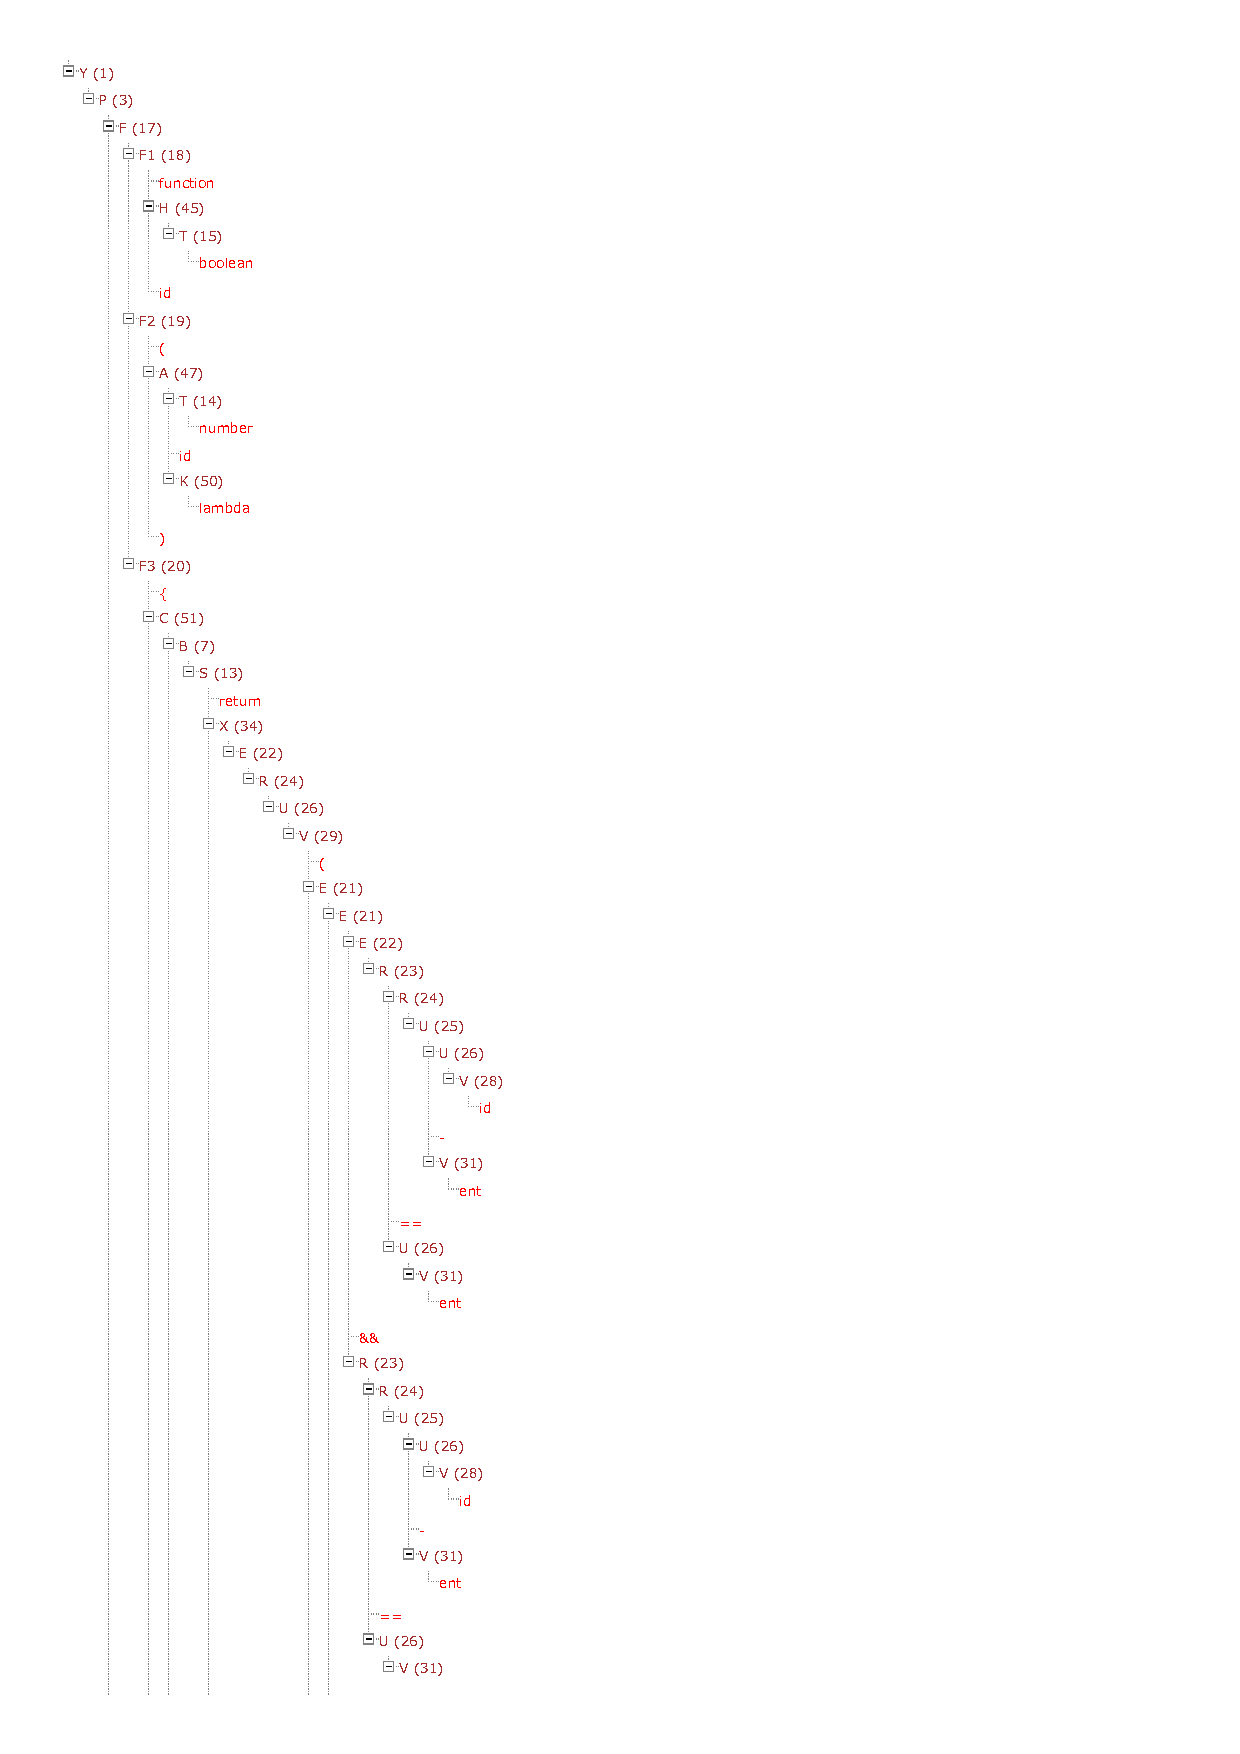
\includepdf[pages=-, landscape=false]{Arbol1.pdf}

\subsubsection{Árbol generado por la segunda prueba correcta}
\label{subsec:arbol2}
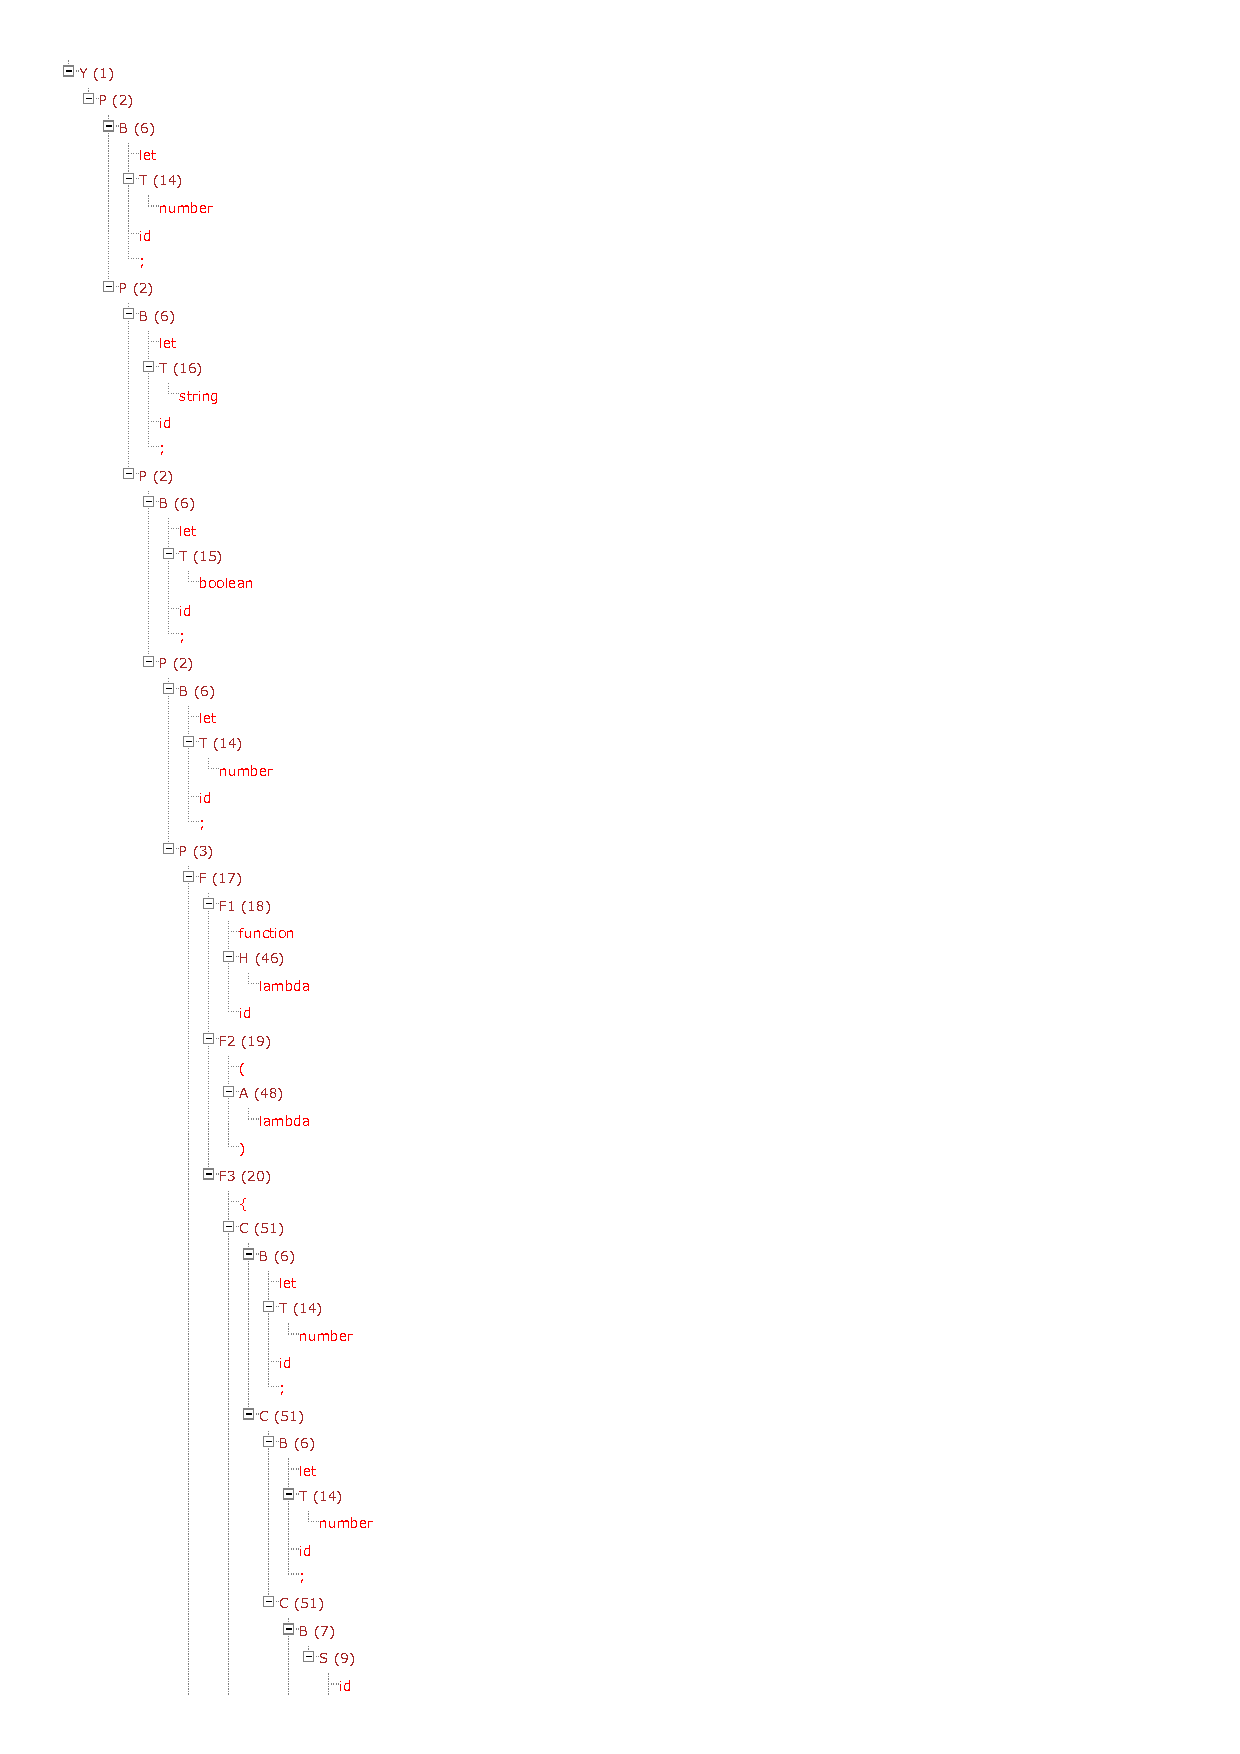
\includepdf[pages=-, landscape=false]{Arbol2.pdf}

\subsubsection{Árbol generado por la tercera prueba correcta}
\label{subsec:arbol3}
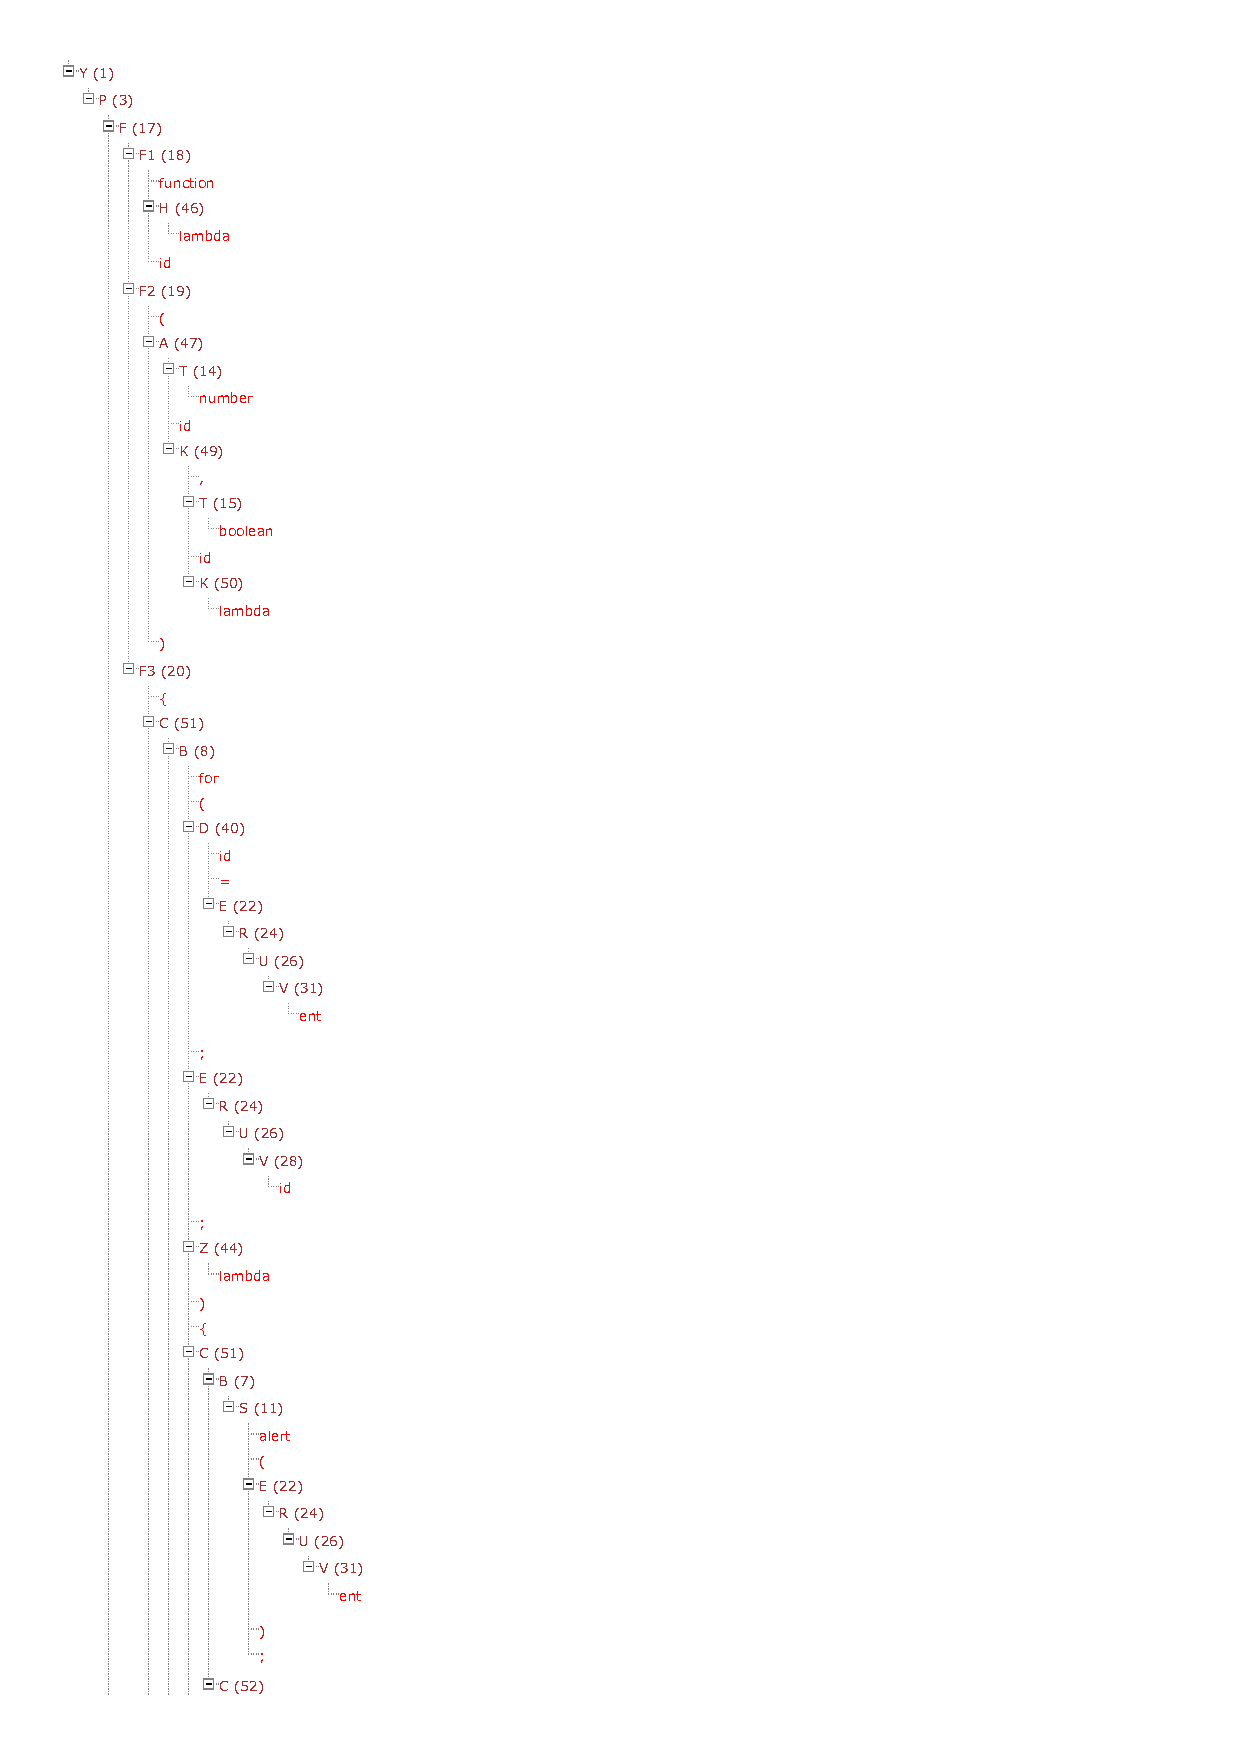
\includepdf[pages=-, landscape=false]{Arbol3.pdf}

\end{document}